\section{Study 2: How review arrangements generate evidence}
\label{sec:actor-review}
\subsection{Research questions and connection to Study 1}
Study 1 prescribes workflow error rates and label quality independently of the arrangement that acquires evidence. Study 2 makes the expressed judgments and final outcomes depend on a human--agent review arrangement. The same private signals may remain available under blind review or be replaced by copied agreement after exposure. Proposers and reviewers instantiate $X$; exposure and order change $\Phi$ and $\Pi$; arbitration changes $L$; and observation retention instantiates $M$. Study 2 was designed and its protocol fixed after Study 1 was completed; it is exploratory.

Three questions organize the study. With individual accuracy fixed, how do private error dependence and exposure-induced copying separately affect decision error and visible agreement? How do these mechanisms change the preferred human--agent arrangement under a fixed budget? Which observations distinguish them, and does continuing to pay for those observations recover its cost?

\subsection{Private errors, copying, and bounded review arrangements}
A binary task has a proposer, agent reviewers, and, in some arrangements, a human arbiter. Humans have private error probability $q_H$; conditional on task truth, their errors are independent of one another and of the agent group. Agents have private error probability $q_A$. With probability $\rho_A$, all agents on a task, including an agent proposer, share one error draw; otherwise their errors are independent. This construction preserves individual accuracy while varying private error dependence.

Motivated by observed sycophancy in multi-agent debate \citep{consensagent}, we isolate copying (echo) without additional task information. Here $\eta_s$ is the probability that an agent reviewer copies an upstream decision from source $s\in\{H,A\}$; otherwise it retains its private judgment. The subscript denotes the upstream actor, so $\eta_H$ describes an agent copying a human. Blind protocols preserve private commitments for aggregation or escalation while retaining any intrinsic error dependence. We compare exposed and blind voting, exposed and blind disagreement-triggered human arbitration, random arbitration of unanimous cases, serial review, and single-actor baselines. Exact enumeration identifies a minimum-error arrangement within the declared candidate catalog and budget; expected cost breaks error ties. Appendix~\ref{app:actor} specifies the joint error law, protocols, costs, parameter grid, and ties.

\subsection{Visible agreement and the placement of human judgment}
For an agent proposer and three agent reviewers, private accuracy of 90\% and $\rho_A=.1$, increasing $\eta_A$ from 0 to .8 raises unanimous agreement with the proposer from 69.06\% to 91.20\%, while majority-decision error rises from 3.52\% to 9.64\%. Conditional on an incorrect proposal, unanimous approval rises from 10.09\% to 59.62\%. Blind voting retains an error rate of 3.52\% under the same private-signal distribution. This comparison illustrates the copying mechanism; agreement alone does not identify its cause. With one agent proposer and one equally capable agent reviewer, $(\rho_A,\eta_A)=(.8,0)$ and $(0,.8)$ produce the same joint distribution of public votes and truth but respond differently to blinding (Appendix~\ref{app:actor}).

\Cref{fig:actor-review} separates copying from pre-existing dependence. With $q_H=.2$, $q_A=.1$, a human-to-agent call-cost ratio of four, blind overhead of .05 per reviewer, and a hard task budget of three human-call units, the minimum-error choice at $\eta_H=\eta_A=.5$ changes from an agent proposer with six blind agent reviewers at $\rho_A=0$ to a human proposer, one blind agent reviewer, and an independent human arbiter on disagreement at $\rho_A=1$.
\begin{figure}[!htbp]
\centering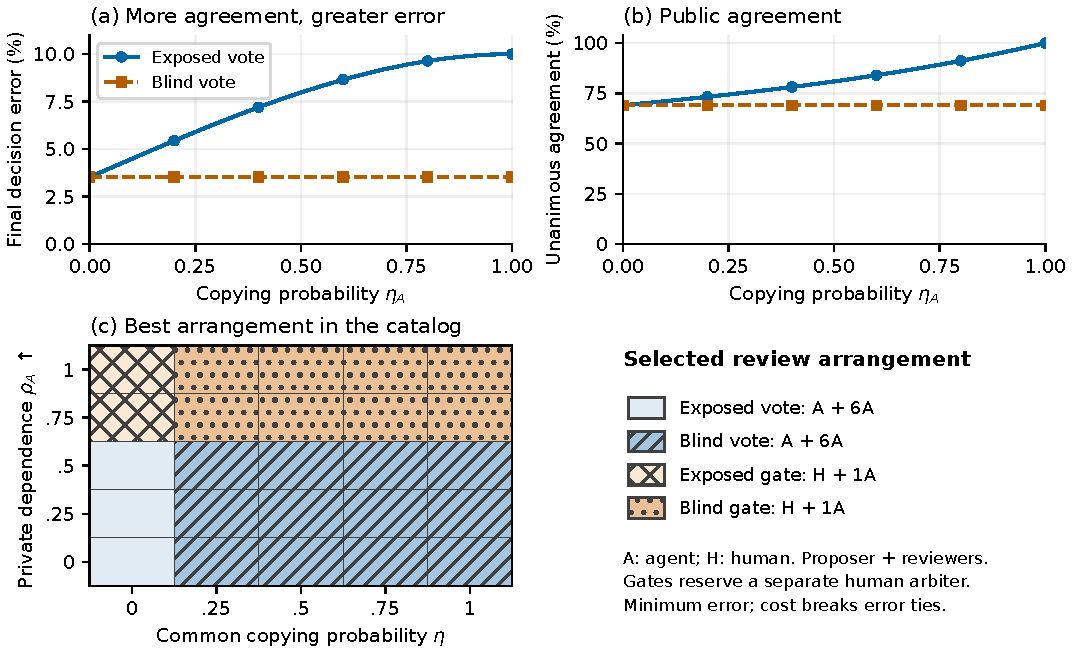
\includegraphics[width=\linewidth]{figures/fig4_actor_review.pdf}
\caption{Study 2: private judgment, upstream exposure, and review organization. (a--b) Final majority-decision error and unanimous agreement for an agent proposer and three agent reviewers, with $q_A=.1$ and $\rho_A=.1$. Exposed reviewers copy with probability $\eta_A$; blind protocols retain private votes. The 21 illustrative values were chosen after the core run. (c) The minimum-error arrangement, with cost breaking error ties, at each dependence and copying setting, for $q_H=.2$, $q_A=.1$, and a hard task budget of three human-call units. Human and agent calls cost 1 and .25; blind commitment adds .05 per reviewer. Gates reserve a separate human arbiter. Dependence increases upward. Colors and hatching identify the selected arrangements; all values are exact expectations.}
\label{fig:actor-review}
\end{figure}
The budget-constrained result concerns the position and authority of human judgment, not just the number of humans. A disagreement-triggered arbiter makes a final decision on selected cases. It does not provide the correct gold label assumed for learning. Under the modeled independent-arbiter rule, randomly overriding unanimous decisions helps only when the arbiter's error probability is below the conditional error probability of those cases. Measurement and decision authority are therefore distinct design variables.

\subsection{Paid observation, retention, and net value}
We compare four fixed observation policies for selecting arrangements with unknown actor parameters. Across 48 rounds, they choose among 58 budget-feasible arrangements under reset, cumulative, or Window 8 memory. They acquire final outcomes only, paired private and post-exposure judgments, or observations from randomized blind and exposed tasks. An \emph{Omit echo} ablation receives the same paired records but sets copying probabilities to zero in its predictions. Six environments, including a copying shift before round 25 and source-dependent copying, use 128 replicate trajectories per condition. All policies share a ceiling on acquisition cost, but purchase different numbers of labels. The cost schedule is separate from Study 1's label-count budget. Observation policies are assigned treatments and do not change during learning.

In High echo with cumulative memory, paired observation achieves mean decision error 1.773\% and net value $.86077$, compared with 9.825\% and $.62323$ for the Omit echo ablation using the same acquired records. The paired net-value difference is $.23755$ (95\% Monte Carlo half-width $.00004$). Randomized exposure reaches 1.782\% error and $.86078$ net value. The fixed blind agent-proposer/three-reviewer baseline has higher error, 3.520\%, but higher net value, $.87140$, because it purchases no continuing learning evidence. Appendix~\ref{app:actor} reports all six environments under cumulative memory; Supplementary Table S5 reports every policy--memory condition and its costs.

Across all six environments, cumulative paired observation has lower error than the fixed blind baseline, but its net value is lower in five. It spends 233.6 acquisition units per round, or $.05703$ per production task after amortization over 4096 tasks. In those five environments this expense exceeds the gain in deployment value, including production call cost; the switch charge is included separately. In Stronger humans, paired observation's net value is $.77306$, compared with $.60740$ for the fixed blind baseline. The result is specific to the stated observation budget, comparator, and amortization scale.

Memory effects depend on the observation policy. In Echo shift, paired observation's full-horizon net values are $.85798$ with reset, $.86255$ with cumulative memory, and $.86274$ with Window 8; cumulative and Window 8 both reach final-16-round error 1.7704\%. For randomized exposure, the corresponding net values are $.85081$, $.85206$, and $.85659$, and final-16-round errors are 2.3212\%, 1.8372\%, and 1.7704\%. Thus finite retention improves adaptation for randomized exposure in this setting, while the cumulative penalty for paired observation is small; the large reversal penalty of Study 1 does not transfer unchanged to every observation procedure.
